\documentclass{scrartcl}
\usepackage[a4paper, total={7in, 10in}]{geometry}
\usepackage{stmaryrd}
\usepackage{amsthm}
\usepackage{amssymb}
\usepackage{amsmath}
\usepackage{algorithm2e}
\usepackage{hyperref}
\usepackage{comment}
\usepackage[french]{babel}
\usepackage{color}
\usepackage{tikz}
\usepackage{graphicx}
\usetikzlibrary{automata, arrows.meta, positioning}
\usepackage{MacrosArt}

%% Generated by ipescript page-labels figs.pdf
%% Do not edit
\newcommand{\ipeFigexcarte}{1}
\newcommand{\ipeFigKKnIpqcompl}{2}
\newcommand{\ipeFigcartetrivperf}{3}
\newcommand{\ipeFigextrivperf}{4}
\newcommand{\ipeFigIpqIrsMap}{5}
\newcommand{\ipeFigIpqIrsItuMap}{6}
\newcommand{\ipeFigtemoinK}{7}
\newcommand{\ipeFigpointabuse}{8}
\newcommand{\ipeFigcographsepind}{9}
\newcommand{\ipeFigfirsttemoin}{10}
\newcommand{\ipeFigfirsttemoinquatriparti}{11}
\newcommand{\ipeFigsecondtemoinquatriparti}{12}

\begin{document}

\title{Stage Map Graphs}

\author{José Lorgeré}

\maketitle

\begin{flushleft}

\section*{Introduction}

\section{Trucs généraux}

\subsection{Résultats et définitions préliminaires}

\begin{def*}[Carte]
    Une carte est une fonction $f : V \rightarrow \mathcal{P}(\mathbb{S}^2)$ telle que pour tout $v \in V$, $f(v)$
    est homéomorphe à $\mathbb{D}^2$ et telle que pour $v \neq u$, $f(u)$ et $f(v)$ sont d'intérieur disjoints. Si
    $f$ forme un recouvrement de $\mathbb{S}^2$, on la dira sans trou, ou complète. On appelera les $f(v)$ régions
\end{def*}

\begin{def*}[Graphe de carte \cite{IntroMap}]
    Un graphe $G = (V, E)$ est de carte s'il existe une carte $f$ sur $V$ telle que $xy \in E$ si et seulement si
    $f(x) \cap f(y) \neq \varnothing$
\end{def*}

\begin{figure}[h]
    \caption{Un graphe, une carte, et un témoin associés à ce dernier}

    \begin{center}
    \begin{tikzpicture}[auto]
        \begin{scope}[every node/.style={circle, draw}]
            
        \node (a) {$a$};
        \node (h) [left = of a] {$h$};
        \node (e) [right = of a] {$e$};
        \node (b) [below = of h] {$b$};
        \node (g) [below = of b] {$g$};
        \node (c) [right = of g] {$c$};
        \node (d) [below = of e] {$d$};
        \node (f) [below = of d] {$f$};
        \end{scope}

        \path
        (a) edge (b) edge (c) edge (d) edge (e) edge (h)
        (b) edge (c) edge (d) edge (h) edge (g)
        (c) edge (d) edge (g) edge (f)
        (d) edge (e) edge (f);
    \end{tikzpicture}
    \hspace*{1.5cm}
    \includegraphics[page=\ipeFigexcarte, scale = 0.5]{figs}
    \hspace*{1cm}
    \includegraphics*[page=\ipeFigfirsttemoin, scale = 0.38]{figs}
    \end{center}
\end{figure}

\begin{theorem}[Caractérisation des graphes de carte]\label{carCarte}
    Un graphe $G = (V, E)$ est de carte si et seulement si il existe $H$ un graphe biparti planaire, de bipartition $V, U$,
    tel que $H^2[V] = G$. Un tel graphe $H$ est appelé graphe témoin de $G$
\end{theorem}

\begin{prop}
    Si $G$ est un graphe de carte, et $H = G[A]$ où $A \subset V$, alors $H$ est un graphe de carte
\end{prop}

\begin{proof}
    On reprend la carte de $G$ où l'on ne garde que les régions identifées aux sommets présents dans $A$
\end{proof}

\begin{def*}[Join]
    Le join de $2$ graphes $G = (V, E)$ et $G' = (V', E')$ est le graphe ayant pour sommet $V'' = V \sqcup V'$ et pour arrêtes
    \[ E'' = E \cup E' \cup \{ xx' \mid x \in V, x \in V' \} \]
    On notera pour tout $n \geq 1$ $K(n, G)$ le join d'un indépendant à $n$ sommets avec le graphe $G$. Plus généralement,
    le join des graphes $G$ et $G'$ sera noté $K(G, G')$. Cette opération étant associative, on se permettra
    d'écrire $K(G, H, L)$ pour désigner le join successif de $G$ à $H$ puis à $L$
\end{def*}

\begin{def*}[Cliques indépendantes]
    Pour tout $k \geq 1$, $n_1, ..., n_k \geq 1$, on dénotera par $I_{n_1, ..., n_k}$ le graphe complémentaire de $K_{n_1, ..., n_k}$.
    Ainsi $I_n$ est l'indépendant à $n$ sommets pour $n$ un entier, et $I_{n_1, ..., n_k}$ pour $k \geq 2$ est composé de $k$
    composantes connexes, qui sont toutes des cliques de tailles $n_1, ..., n_k$
\end{def*}

\begin{def*}[Union disjointe]
    L'union disjointe de deux graphes $G = (V, E)$ et $G' = (V', E')$ est le graphe ayant pour sommets $V \cup V'$ et pour arrêtes
    $E \cup E'$. On notera cette dernière $I(G, G')$. Cette opération étant également associative, on se permettre de reprendre la
    convention du join.\\
    On notera pour tout $n \geq 1$, $I(n, G)$ l'union disjointe d'une clique à $n$ sommets et du graphe $G$.
\end{def*}

\subsection{Premières obstructions à l'existence de cartes}

\begin{lem}\label{CNSK33}
    Un graphe $G$ a pour mineur $K_{3,3}$ si et seulement si il existe $6$ sommets, $s_1, s_2, s_3, t_1, t_2, t_3$ et des chemins
    $P_{i,j}$ de $s_i$ à $t_j$ pour tout $i, j$ tels que
    \begin{itemize}
        \item Pour tout $i \neq i', j \neq j'$, $P_{i',j'}$ et $P_{i, j}$ ne se rencontrent pas
        \item Pour tout $i$, $s_i$ et $t_i$ ne sont sommet intermédiaire d'aucun des chemins
        \item Si deux de ces chemins se rencontrent, leur intersection est également un chemin
    \end{itemize}
\end{lem}

\begin{proof}
    Supposons que $G$ possède un mineur $K_{3,3}$. Alors il existe des ensembles de sommets connexes, disjoints, $S_1, S_2, S_3, T_1, T_2, T_3$
    tels qu'une fois contractés, le graphe induit par ces ensembles aie pour sous graphe $K_{3,3}$. Soient $s_i \in S_i$ et $t_i \in T_i$
    pour $i \in \{1, 2, 3\}$. Comme on a une arrête de $S_i$ à $T_j$ pour tout $i,j$, il existe des sommets $s'_i \in S_i$ et $t'_j \in T_j$
    tels que $s'_i t'_j \in E$. En se donnant un chemin de $s_i$ à $s'_i$ puis de $t'_j$ à $t_j$, on construit alors des chemins
    $P_{i,j}$ comme décrits dans l'énoncé. Si $i \neq i'$, $j \neq j'$, les chemins $P_{i,j}$ et $P_{i',j'}$ sont à valeurs dans des
    ensembles disjoints et ne se rencontrent donc pas. La deuxième condition est vérifiée pour les mêmes raisons. Pour la troisième,
    si un chemin de $s_i$ à $t_j$ rencontre un chemin de $s_i$ à $t_{j'}$ en un sommet intermédiaire, cette intersection se fait nécessairement
    dans $S_i$. On modifie alors le chemin $P_{i,j'}$ de sorte à ce qu'il coincide avec $P_{i,j}$ jusqu'à sa dernière intersection avec ce dernier
    dans $S_i$. On raisonne de manière similaire pour $P_{i,j}$ et $P_{i',j}$
    \\~\\
    Supposons à présent qu'il existe de tels $s_i$ et $t_i$ et de tels chemins $P_{i,j}$. On se restreint au sous graphe constitué des
    chemins $P_{i,j}$. Soient $i,j \in \{1,2,3\}$.
    Supposons que $P_{i,j}$, hors extérmités, ne soit pas disjoint de tout les autres chemins. On note
    $P_{i,j} = \{s_i = v_1, v_2, ..., v_l = t_j\}$ dans l'ordre de parcours, et on se donne
    \begin{equation*}
    \begin{split}
        p &= \min \{ k \in \llbracket 1, l \rrbracket \mid \exists i' \neq i, v_k \in P_{i',j}\}\\
        q &= \max \{ k \in \llbracket 1, l \rrbracket \mid \exists j' \neq j, v_k \in P_{i, j'} \}
    \end{split}
    \end{equation*}
    L'hypothèse faite sur les chemins permet d'affirmer que les deux ensembles décrits sont les seules intersections possibles de $P_{i,j}$
    avec d'autres chemins.\\
    Montrons que $p > q$ : on se donne les $i'$ et $j'$ correspondants. Comme l'intersection de deux chemins reste un chemin, et que $P_{i,j'}$
    contient à la fois $s_i$ et $v_q$, les sommets $v_1, ..., v_q$ font tous partie de $P_{i,j'}$. De même, $v_p, ..., v_l$ font partie
    de $P_{i',j}$. Supposons maintenant par l'absurde que $p \leq q$. On déduit des remarques précédentes que les sommets $v_p, ..., v_q$
    font partie de $P_{i,j'}$ et $P_{i',j}$, hors ces chemins ne s'interesctent pas par hypothèse, absurde.\\
    On contracte alors tout les sommets de $v_1$ à $v_p$ et ceux de $v_q$ à $v_l$ comme il existe un chemin les reliant tous. Puisque
    $p > q$ et que les sommets de départs et d'arrivée ne sont pas présents sur les chemins hors extrémités,
    on conserve bien des chemins de $s_i$ à $t_{j'}$ et de $s_{i'}$ à $t_j$. Après cette opération, le nouveau chemin $P_{i,j}$ est disjoint
    de tout les autres. On répète alors cette opération pour tout $i,j$.\\
    Une fois cela fait, on obtient des chemins tous disjoints de tout $s_i$ à tout $t_j$, ne reste plus qu'à contracter ces chemins afin
    d'obtenir un $K_{3,3}$.
\end{proof}


\begin{prop}\label{K3G}
    Soit $G$ un graphe à $3$ sommets. $K(3, G)$ n'est pas un graphe de carte
\end{prop}

\begin{proof}
    Supposons par l'absurde que $K(3, G)$ est un graphe de carte. On se donne alors $H$ vérifiant toutes les propriétés
    du théorème \ref{carCarte}. On note pour tout $v_i$, sommet indépendant de $K(3, G)$, $N_i$ son voisinage dans $H$
    incluant $v_i$. Notons que pour $i \neq j$, $N_i$ et $N_j$ sont disjoints comme $v_i$ et $v_j$ sont indépendants.
    Comme les chemins de $v_i$ aux sommets de $G$ n'empruntent que des sommets de $N_i$, mis à part le sommet de $G$,
    les hypothèses du lemme \ref{CNSK33} sont vérifiées. $H$ a donc pour mineur $K_{3,3}$, absurde par planarité.
    $K(3, G)$ n'est donc pas un graphe de carte.
\end{proof}

Notons toutefois que $K(2, G)$ lui est un graphe de carte, et que le join de $2$ graphes à $3$ sommets tous deux non indépendants
est de carte également. Cela pourrait laisser à penser que, comme pour les graphes planaires, les graphes $K(3, G)$ seraient des
contre exemples "fondamentaux". Ce n'est en fait pas le cas, la proposition suivante montrant qu'un graphe n'a pas besoin
d'avoir $3$ indépendants pour ne pas être de carte
\\~\\
(Trouver une preuve plus simple de $K_{2,2,2,2}$, topologiquement ça a l'air izy)

\begin{prop}\label{K2222}
    $K_{2,2,2,2}$ n'est pas un graphe de carte
\end{prop}

\begin{proof}
    On numérote les sommets de $1$ à $8$, tels que $\{v_1,v_2\}$, $\{v_3,v_4\}$, $\{v_5,v_6\}$, $\{v_7,v_8\}$ soient les indépendants.
    On suppose par l'absurde que $K_{2,2,2,2}$ est un graphe de carte, on s'en donne donc un témoin $H$. On le suppose même minimal pour
    la relation de sous graphe.\\
    Notons d'abord que les voisinages de $v_1$ et $v_2$ dans $H$ sont disjoints, ces deux sommets étant indépendants. Cela vaut
    aussi pour toutes les autres paires indépendantes. Ainsi, pour tout $u \in N(v_i)$, $u$ n'est voisin que d'au plus un élement de
    chaque paire. Ainsi les sommets de $U$ sont de degré au plus $4$. On construit à présent un mineur $K_{3,3}$ de $H$
    \\~\\
    Notons que comme $K_{2,2,2,2}$ n'est pas planaire, au moins un sommet de $H$ dans $U$ est de degré au moins $4$. Les remarques
    précedentes font que ce sommet est de degré exactement $4$. Notons le $u$, et supposons quitte à renommer que ses voisins
    sont $v_1, v_3, v_5, v_7$. Soit $i \in \{4, 6, 8\}$. Notons $p, q, r$ les voisins de $v_2$ donnant un chemin de longueur
    $2$ respectivement à $v_3, v_5, v_7$. Depuis $v_i$ on construit un chemin vers $v_{i-1}$ en exploitant un sommet $v_j \in V$ intermédiaire
    tel que $j \notin \{1, 2, 3, 5, 7, i\}$. Les autres chemins depuis $v_i$ sont ceux de longueurs $2$ donnés par le fait que $H$ soit
    un témoin de $K_{2,2,2,2}$. On note alors $q', p', r'$ les voisins de $v_i$ participant à chacun de ces $3$ chemins
    ordonnés de même manière que $p, q, r$. On notera $s'$ le sommet de $U$ venant après $v_j$ dans le chemin de $v_i$ à $v_{i-1}$\\
    Une disjonction de cas basée sur les remarques faites sur le degré des sommets et la minimalité de $H$ montre
    que l'on peut choisir $i$ et $j$ tels que les chemins de $v_i$ et $v_2$ à $v_3, v_5, v_7$ se rencontrent selon
    les hypothèse du lemme \ref{CNSK33}.
    \\~\\
    On considère les sommets $v_1, v_2, v_i, v_3, v_5, v_7$ et les chemins donnés précedemment (le chemin depuis $v_1$ aux autres est de longueur
    $2$ et utilise $u$). $u$ étant de degré $4$ donc maximal, et par ce qui précède, ces sommets vérifient les hypothèses du lemme
    \ref{CNSK33}. Donc $H$ n'est pas planaire. Absurde
\end{proof}

\begin{prop}\label{K222K5}
    $K(2,2,2,K_5)$ n'est pas un graphe de carte
\end{prop}

\begin{proof}
    Supposons par l'absurde qu'il le soit, on s'en donne alors un témoin $H$. On numérote les indépendants $\{v_1, v_2\}, \{v_3, v_4\}, \{v_5, v_6\}$
    et $a_1, ..., a_5$ les sommets de la clique $K_5$. On pose $S \subset V \cup U$ le sous ensemble composé de $a_1, ..., a_5$, des sommets
    de $U$ tels que tout leurs voisins soient parmi $a_1, ..., a_5$, et des sommets de $U$ de degré $2$ tels que l'un des deux voisins
    est parmi $a_1, ..., a_5$.\\
    $H - S$ est un témoin de $K_{2,2,2}$. On écrit alors $V \cup U \backslash S = \{v_1, ..., v_6\} \cup U'$.
    Par des arguments similaires à la proposition précédente, les sommets de $U'$ sont de degré au plus $3$ dans $H - S$.
    Pour tout $i \in \{1, ..., 5\}$, $a_i$ étant adjacent à tout les $v_1, ..., v_6$ dans $K(2,2,2,K_5)$, on en déduit que dans le plongement
    de $H$, $a_i$ est placé dans une face de $H-S$ telle que, en notant $A_i$ les sommets adjacents à cette dernière, $RA(A_i) = \{v_1, ..., v_6\}$.\\
    Montrons à présent que $a_i$ a au moins $3$ voisins : si il n'en avait que $2$, ces voisins que l'on note
    $u$ et $u'$ ont respectivement pour voisins dans $H - S$ $v_1, v_3, v_5$ et $v_2, v_4, v_6$. On considère les sommets $v_1, v_2, v_3, a_i, v_5, v_6$
    et les chemins suivants : de $v_1$ et $v_3$ à $a_i$, on utilise $u$, de $v_2$ à $a_i$ on utilise $u'$, puis pour le reste on prend des sommets
    intermédiaires quelconques. Ces derniers vérifient les hypothèses du lemme \ref{CNSK33} par indépendances et comme $u \neq u'$, absurde comme $H$
    est planaire, donc $a_i$ a bien au moins $3$ voisins. Cela permet alors d'affirmer que chaque face vérifiant les hypothèses précédentese
    ne peut pas accueillir plus d'un $a_i$ par planarité. Il y a donc $5$ faces vérifiant ces hypothèses.
    \\~\\
    Considérons une face vérifiant les hypothèse : cette dernière ne peut avoir les $6$ sommets de $K_{2,2,2}$ sur son bord car alors il n'y aurait
    qu'au plus une seule autre face pouvant vérifier les hypothèses pour des raisons de planarité (on peut par exemple y trouver un mineur
    $K_{3,3}$). De même si cette dernière contient $5$ sommets. Si cette dernière contient $4$ sommets, alors par les remarques précédentes
    sur le nombre de voisins minimal de $a_i$, les deux sommet de $U'$ sur le bord de degré $3$ ont des voisinages non disjoints. Cela
    conduit au fait d'avoir une autre face ayant plus de $5$ sommets de $K_{2,2,2}$ sur son bord, encore impossible. Donc toutes les
    faces ont au plus $3$ sommets de $K_{2,2,2}$ sur leur bord. En fait il y en a exactement $3$, sinon on ne peut vérifier l'hypothèse comme
    les sommets de $U'$ sur le bord sont de degré au plus $3$ et ne peuvent avoir des voisinages disjoints. On déduit également de cela que tout les sommets
    de $U'$ sur les bords des faces sont de degré exactement $3$ afin d'avoir $RA(A_i) = \{v_1, ..., v_6\}$.
    \\~\\
    $H-S$ est alors nécessairement le graphe illustré figure \ref{temoinK222}, quitte à renuméroter.
    Ce graphe a $4$ faces. Absurde, $K(2,2,2,K_5)$ n'est donc pas de carte.
\end{proof}

\begin{figure}[h]
    \caption{Le graphe $H - S$ de la proposition \ref{K222K5}}\label{temoinK222}
    \begin{center}
        \includegraphics[page=\ipeFigtemoinK, scale = 0.5]{figs}
    \end{center}
\end{figure}

Notons que $K_{2,2,2}$ est toutefois un graphe de carte. Ces deux propositions donnent alors des conditions nécessaires au fait
de posséder une carte : en effet les graphes de carte étant stables par sous graphe induit, ces derniers ne peuvent alors
posséder ni $K(3, G)$ ni $K_{2,2,2,2}$ parmi ces derniers. Ces conditions ne sont pas suffisantes : une subdivision
de $K_{3,3}$ quelconque n'est pas un graphe de carte par des arguments similaires à la proposition \ref{K3G}

\subsection{Cartes et connexités}\label{cartesetconnex}

La propriété pour un graphe d'admettre une carte a des interactions avec la connexité de ce dernier, et à quel point cette connexité
est forte. Par exemple, un graphe est de carte si et seulement si chacune de ses composantes connexes l'est, ce qui peut se montrer
facilement à l'aide d'un témoin. Dans toute la suite, on considèrera alors que tout les graphes que l'on cherche à étudier sont connexes.
\\~\\
Les graphes admettant une carte complète ont des propriétés de connexité particulière : on peut en effet montrer par des arguments
topologiques (en exploitant le fait que chaque région est homéomorphe à un disque) qu'un graphe admettant une telle carte
est nécesairement $2$-connexe. Ceci couplé à la proposition suivante permet de dire que l'on peut accéder à toutes les propriétés
intéressantes des cartes en ne regardant que celles $2$-connexes

\begin{prop}\label{suffbiconn}\cite{FptMap}
    Un graphe $G$ est de carte si et seulement si toutes ses composantes $2$-connexes le sont
\end{prop}

On peut par exemple en déduire qu'un block graph, c'est à dire un graphe dont les composantes $2$-connexes sont des cliques,
est alors toujours un graphe de carte, et admet une carte complète si et seulement si ce dernier est une clique\\
On pourrait alors se demander, à la lumière des exemples de $K(3,G)$ et $K_{2,2,2,2}$ si un graphe n'étant pas $3$-connexe
peut ne pas être de carte. Le graphe donné par un $K_{3,3}$ auquel on ajoute un sommet de degré $2$ n'est pas $3$-connexe
et n'est pas de carte.
\\~\\
La $3$-connexité jouant un rôle important dans la suite, on se propose de voir comment on peut se ramener à l'étude des
graphes $3$-connexes à partir d'un graphe $2$-connexe \cite{3connComp}.\\
Si $\{x,y\} \subset V$ est un séparateur d'un graphe $G$ $2$-connexe, on note $C_1, ..., C_k$ les composantes connexes de
$G - \{x,y\}$. Pour tout $i$, on note $G_i$ le graphe induit par $C_i \cup \{x,y\}$ auquel on a rajouté l'arrête $xy$.
$G_i$ est $2$-connexe. Si $G_i$ n'est pas $3$-connexe, il existe alors séparateur de taille $2$ et on peut ainsi recommencer
ce processus. En répétant ce processus, on finit par obtenir un ensemble de graphes $3$-connexes. La donnée de ces graphes finaux
ainsi que celle des $2$-séparateurs permettant de les obtenir sera appelée une décomposition $3$-connexe de $G$.
Les graphes $3$-connexes finaux seront appelés des composantes $3$-connexes de $G$ associés à cette décomposition.

\begin{prop}\label{3connCompCarte}
    Soit $G$ un graphe de carte $2$-connexe. Pour toute décomposition $3$-connexe de $G$, ses composantes sont des graphes de carte
\end{prop}

\begin{proof}
    On montre uniquement que, étant donné un séparateur $\{x,y\}$ de $G$, tout les $G_i$ associés sont des graphes de carte.
    Si $xy$ est une arrête de $G$, alors chaque $G_i$ est un sous graphe induit de $G$ et on a ce qu'on veut. Sinon, on construit une
    carte à $G_i$ à partir de celle de $G$ : comme $\{x,y\}$ est un séparateur, il existe au moins une autre composante connexe de
    $G - \{x,y\}$, que l'on note $C_j$, $j \neq i$. $x$ et $y$ étant reliés à $C_j$, il existe un chemin de $x$ à $y$ dans $C_j$.
    On se donne un témoin $H$ associé à $G$. L'existence de ce chemin dans $G$ donne un chemin dans $H$ de $x$ à $y$, jamais voisin
    d'un sommet de $C_i$ sauf en $x$ et $y$. En considérant le sous graphe de $H$ obtenu en ne considérant que le voisinage de $C_i$ et le chemin
    de $x$ à $y$ évoqué, on peut en contractant des arrêtes du chemin obtenir un témoin de $G_i$
\end{proof}

\section{Algorithmes}

On discutera ici d'abord du problème de reconnaissance des graphes de carte, restreint à des sous classes particulières, puis l'on s'intéressera

\subsection{Cas des graphes trivialement parfaits}

Un graphe $G$ sera dit trivialement parfait s'il ne contient pas les graphes $P_4$ et $C_4$ en sous graphe induit.
Il est équivalent de les définir comme des graphes d'intervalles particuliers. Un graphe trivialement parfait est le graphe
d'intersection d'un ensemble d'intervalles "emboîtés" : si $I$ et $J$ sont deux intervalles représentant des sommets de $G$,
si $I \cap J \neq \varnothing$, alors $I \subset J$ ou inversement. Un exemple d'une telle représentation est donné figure
\ref{extrivperf}\\
Cette définition par les intervalles permet de voir facilement que l'unique séparateur minimal d'un graphe trivialement parfait $G$ est
composé de l'ensemble des sommets universels de $G$ (un sommet universel étant un sommet adjacent à tout les sommets du graphe). Ainsi
$G$ est $3$-connexe si et seulement si il possède au moins $3$ sommets universels.

\begin{figure}[h]
    \caption{Un graphe trivialement parfait et sa représentation par des intervalles emboîtés}\label{extrivperf}
    \begin{center}
        \begin{tikzpicture}[auto]
        \begin{scope}[every node/.style={circle, draw}]
            
        \node (u) {$\0$};
        \node (a0) [above left = 7mm and 30mm of u] {$\0$};
        \node (a1) [above = 7mm of u] {$\0$};
        \node (a2) [above right = 7mm and 30mm of u] {$\0$};
        \node (b00) [above = of a0] {$\0$};
        \node (b10) [above left = 7mm and 5mm of a1] {$\0$};
        \node (b11) [above right = 7mm and 5mm of a1] {$\0$};
        \node (c000) [above left = 7mm and 3mm of b00] {$\0$};
        \node (c001) [above right = 7mm and 3mm of b00] {$\0$};
        \end{scope}

        \path
        (u) edge (a0) edge (a1) edge (a2) edge (b00) edge (b10) edge (b11) edge (c000) edge (c001)
        (a0) edge (b00) edge (c000) edge (c001)
        (a1) edge (b10) edge (b11)
        (b00) edge (c000) edge (c001);
    \end{tikzpicture}
    \hspace*{1cm}
    \includegraphics[page=\ipeFigextrivperf, scale = 0.85]{figs}
    \end{center}
\end{figure}

\subsubsection{Cas $3$-connexe}

On se fixe pour la suite un graphe $G$ trivialement parfait $3$-connexe

\begin{lem}\label{trivPerfind}
    Si $G$ a $3$ sommets indépendants, il n'est pas de carte
\end{lem}

\begin{proof}
    Un tel graphe contient $K(3, K_3)$ parmi ses sous graphes induits, par les remarques précédentes
\end{proof}

Supposons que $G$ ne soit pas une clique.
On peut déduire de ce lemme que le séparateur minimal de $G$ le sépare en $2$ composantes connexes. Notons que ce séparateur est une
clique de taille au moins $3$. Notons $C_1$ et $C_2$ les $2$ composantes connexes séparées par ce séparateur. Le lemme
\ref{trivPerfind} permet également de déduire que $C_1$ et $C_2$ sont des cliques : en effet si $C_1$ n'est pas une clique,
il contient $2$ sommets indépendants. On a donc un indépendant de taille $3$ constitué de ces $2$ sommets et d'un sommet de $C_2$.
On en déduit le lemme suivant :

\begin{lem}\label{trivPar3conn}
    $G$ est de carte si et seulement c'est une clique ou un $K(K_n, I_{p,q})$ avec $n \geq 3$. De plus, la carte
    donnée est complète
\end{lem}

\begin{proof}
    Le sens direct a déjà été traité précedemment.\\
    Pour le sens réciproque, toute clique admettant une carte complète, on se concentre sur le second cas. On construit
    alors une carte complète pour $K(K_n, I_{p,q})$ comme illustré figure \ref{KKnIpqmap}
\end{proof}

\begin{figure}[h]
    \caption{Carte complète pour $K(K_n, I_{p,q})$}\label{KKnIpqmap}
    \begin{center}
        Le séparateur en "donut" représente la clique $K_n$\\
        \includegraphics[page=\ipeFigKKnIpqcompl, scale = 0.4]{figs}
    \end{center}
\end{figure}

\subsubsection{Cas général}

On s'intéresse à présent au cas où $G$ est $2$-connexe, qui conclura l'analyse des graphes trivialement parfaits par la proposition
\ref{suffbiconn} et le fait qu'un graphe à carte complète est nécessairement $2$-connexe.\\
Comme précedemment, la $2$-connexité de $G$ impose l'existence de $2$ sommets universels. S'il y en a $3$, la question
a déjà été réglée précédemment car $G$ est alors $3$-connexe. Notons que le séparateur minimal étant unique et universel,
$G$ n'a qu'une seule décomposition $3$-connexe. On parlera alors simplement de composantes $3$-connexes de $G$ sans préciser
de décomposition.

\begin{theorem}\label{maptrivperf}
    Un graphe $G$ trivialement parfait $2$-connexe est de carte si et seulement si chacune de ses composantes $3$-connexe est de carte.
    De plus la carte de $G$ construite est complète.
\end{theorem}

\begin{proof}
    Si $G$ est de carte, toutes ses composantes $3$-connexes sont de carte par la proposition \ref{3connCompCarte}\\
    Pour le sens réciproque, le lemme \ref{trivPar3conn}, nous donne la forme des composantes $3$-connexes de $G$.
    Notons $C_1, ..., C_k$ les composantes $3$-connexes de $G$. On construit alors une carte comme suit :
    on place $2$ régions associées aux $2$ universels, $u$ et $v$, de $G$, que l'on fait se rencontrer en $k+1$ chemins disjoints.
    Ainsi après retrait de ces $2$ régions, la sphère est séparée en $k$ composantes connexes.\\
    Si $C_i$, $1 \leq i \leq k$, est une clique, on place dans une des $k$ composantes connexes encore libre une clique
    remplissant entièrement cette composante, portée par un point de rencontre entre $u$ et $v$. Sinon $C_i$ est
    de la forme $K(K_n, I_{p,q})$, $n \geq 3$. On représente alors les sommets distincts de $u$ et $v$ formant le $K_n$
    par une clique séparant la composante en deux, de telle sorte à ce que chaque partie ait accès à un point portant
    cette clique. On remplit ensuite chaque partie par une clique portée par un point porteur de la clique $K_n$.
\end{proof}

\begin{figure}[h]
    \caption{Illustration de la construction du théorème \ref{maptrivperf}}
    \begin{center}
        Dans le "trou" de gauche, on a représenté un $K(K_n, I_{p,q})$, alors que dans le "trou" extérieur et de droite,
        on a représenté des cliques
        \\~\\
        \includegraphics[page=\ipeFigcartetrivperf, scale = 0.6]{figs}
    \end{center}
\end{figure}

Notons alors que les graphes trivialement parfaits de carte sont exactement les graphes ne possédant pas $C_4, P_4, K(3, K_3)$ parmi
leur sous graphes induits : en effet, un graphe trivialement parfait de carte vérifie cette condition, et réciproquement, un graphe
n'ayant pas ces $3$ sous graphes induits sera de carte car tout le raisonnement est basé sur le seul lemme \ref{trivPerfind}
\\~\\
(A rediscuter avec la possibilité de juste passer en force par les sous graphes interdits)
On en déduit alors un algorithme en temps polynômial décidant si un graphe $G$ trivialement parfait est de carte : on commence
par séparer $G$ en ses composantes connexes puis $2$-connexes, puis $3$-connexes.
\\~\\
Puis, afin de décider si les composantes $3$-connexes ont bien la forme souhaitée, on emploie l'algorithme suivant : on liste les cliques
max de la composante, si la composante elle même est une clique max, il n'y a alors qu'une seule clique max et ce cas est donc
vu dès la première clique listée. On renvoie alors une réponse positive. Si il n'y a que $2$ cliques max, chaque sommet étant
dans au moins une clique max, ces deux dernières recouvrent la composante $3$-connexe. La $3$-connexité impose que ces deux dernières
se rencontrent en au moins $3$ points, le graphe est alors de la forme $K(K_n, I_{p,q})$, les $2$ cliques max ayant $n+p$
et $n+q$ sommets chacune, la clique $K_n$, $n \geq 3$ étant formée des sommets communs aux deux cliques max. On renvoie alors
aussi une réponse positive. Si il y a plus de $3$ cliques max, on renvoie une réponse négative.

\subsection{Cas des cographes}

Une classe plus large que celle des graphes trivialement parfaits est celle des cographes : un graphe est un cographe s'il ne possède pas
$P_4$ parmi ses sous graphes induits. Il est équivalent de les définir comme le plus petit ensemble de graphes contenant le sommet, stable par
union disjointe et join \cite{cotrees}. Cette dernière caractérisation s'avèrera plus intéressante pour l'étude.\\

En effet cette dernière donne lieu à une représentation des cographes par des arbres enracinés : il s'agit en fait d'utiliser l'arbre
enraciné des opérations, de join (étiquetté par $1$) et union disjointe (étiquettée par $0$), nécessaires afin d'obtenir le cographe en question,
où les feuilles sont donc les sommets du graphe. Deux sommets sont alors adjacents si et seulement si leur plus petit ancêtre commun est un $1$.
Les opérations de join et union disjointe étant associatives, il est alors possible de compacter le coarbre de telle sorte à ce qu'un noeud
$1$ ne puisse avoir comme enfant que des noeuds $0$ ou des sommets et de même pour $0$. La représentation devient alors unique pour un cographe
donné, on appelle cet arbre le coarbre associé au cographe, la figure \ref{excographe} donne un exemple d'un cographe et de son coarbre \cite{cotrees}.
On remarquera que les opérations de join et union disjointe étant au moins binaires, tout les noeuds internes ont au moins $2$ enfants. 

\begin{figure}[h]
    \caption{Le graphe $K(2,I(1,K_{2,2}))$ et son coarbre}\label{excographe}
    \vspace*{0.5cm}
    \begin{center}
        \begin{tikzpicture}[auto]
            \begin{scope}[every node/.style={circle, draw}]
                \node (1) {$v_1$};
                \node (2) [left = of 1] {$v_2$};
                \node (3) [below left = of 2] {$v_3$};
                \node (4) [below = of 3] {$v_4$};
                \node (5) [below right = of 4] {$v_5$};
                \node (6) [right = of 5] {$v_6$};
                \node (a) [below left = 4mm and 10mm of 3] {$a$};

                \node (0) [right = 70mm of 1] {$1$};
                \node (00) [below left = 7mm and 15mm of 0] {$0$};
                \node (01) [below right = 7mm and 15mm of 0] {$0$};
                \node (000) [below left = 7mm and 7mm of 00] {$1$};
                \node (001) [below right = 7mm and 7mm of 00] {$a$};
                \node (010) [below left = 7mm and 7mm of 01] {$v_3$};
                \node (011) [below right = 7mm and 7mm of 01] {$v_4$};
                \node (0000) [below left = 7mm and 7mm of 000] {$0$};
                \node (0001) [below right = 7mm and 7mm of 000] {$0$};
                \node (00000) [below left = 7mm and 1mm of 0000] {$v_1$};
                \node (00001) [below right = 7mm and 1mm of 0000] {$v_2$};
                \node (00010) [below left = 7mm and 1mm of 0001] {$v_5$};
                \node (00011) [below right = 7mm and 1mm of 0001] {$v_6$};
            \end{scope}

            \path
            (1) edge (3) edge (4) edge (5) edge (6)
            (2) edge (3) edge (4) edge (5) edge (6)
            (a) edge (3) edge (4)
            (3) edge (5) edge (6)
            (4) edge (5) edge (6)
            (0) edge (00) edge (01)
            (00) edge (000) edge (001)
            (000) edge (0000) edge (0001)
            (0000) edge (00000) edge (00001)
            (0001) edge (00010) edge (00011)
            (01) edge (010) edge (011);

        \end{tikzpicture}
    \end{center}
\end{figure}

\subsubsection{Connexités et coarbres}

On discutera ici de comment se manifeste les différentes propriétés de connexité des cographes au niveau de leur coarbre associé. Le lemme
suivant caractérise la connexité par la racine de du coarbre

\begin{lem}
    Un cographe $G$ est connexe si et seulement si son coarbre $T$ a pour racine un noeud $1$
\end{lem}

Dont on peut déduire la proposition suivante

\begin{prop}\label{sepcographe}
    Soit $G$ un cographe connexe et $T$ son coarbre. Notons $T_1, ..., T_k$ les sous arbres de $T$ enracinés en les enfants de la racine de $T$.
    Les séparateurs minimaux de $G$ sont exactement les $\displaystyle \bigcup_{i \neq j} V(T_i)$ où $j$ parcourt l'ensemble des indices de $1, ..., k$
    tels que $T_i$ ne soit pas une feuille
\end{prop}

\begin{proof}
    Les ensembles décrits sont bien des séparateurs : notons $\displaystyle S_j = \bigcup_{i \neq j} V(T_i)$ pour un tel $j$. $G - S_j$ peut être
    représenté par l'arbre $T$ où l'on a retiré les sous arbres $T_i, i \neq j$. Mais alors la racine n'a plus qu'un enfant et sa représentation est donc
    inutile. Donc $G - S_j$ peut être représenté par $T_j$, il s'agit même de son coarbre. Or $T_j$ a un $0$ a sa racine comme ce n'est pas une feuille.
    \\~\\
    Soit $S$ un séparateur. Soient $s, t$ deux sommets séparés par $S$. Le plus petit ancêtre commun de $s$ et $t$ dans $T$
    est donc un noeud $0$. $T$ étant le coarbre de $G$, connexe, $0$ a pour parent un noeud $1$. Tout $r$ descendant de ce noeud, n'étant pas dans le
    sous arbre contenant $s$ et $t$ fournit un chemin de longueur $3$ de $s$ à $t$. En particulier, en notant $j$ l'indice du sous arbre de la racine
    contenant $s$ et $t$, $T_j$ n'est pas une feuille et $S$ contient alors $V(T_i)$ pour tout $i \neq j$. Donc $S_j \subset S$. On montre
    alors que les $S_j$ sont des séparateurs minimaux, et que ce sont les seuls
\end{proof}

\begin{cor}\label{coarbrekconn}
    Un cographe $G$ est $k$-connexe si et seulement si pour tout $j$ tel que $T_j$ n'est pas une feuille, $\sum_{i \neq j} |V(T_i)| \geq k$
\end{cor}

On mènera alors une étude similaire aux graphes trivialement parfaits, en se concentrant d'abord sur les cographes à forte connexité pour ensuite
généraliser les résultats

\subsubsection{Structure des cographes de carte}

\begin{theorem}\label{cograph3conn}
    Soit $G$ un cographe $3$-connexe. $G$ est de carte si et seulement si son coarbre est de hauteur inférieure à $4$ et que l'une des deux
    conditions est remplie :
    \begin{itemize}
        \item La racine a au plus $2$ fils étiquettés $0$
        \item La racine a $3$ fils étiquettés $0$ et au plus $4$ autres fils 
    \end{itemize}
\end{theorem}

\begin{proof}
    Supposons $G$ de carte. Notons $T$ son coarbre. Il n'existe aucun noeud $1$ de $T$ ayant plus de $4$ fils $0$ : en effet chaque fils $0$
    possède au moins $2$ descendants, on pourrait alors construire un sous graphe induit $K_{2,2,2,2}$ ce qui est impossible comme $G$ est de carte.
    Si la racine a $3$ fils $0$ et au moins $5$ fils sommets, on peut construire un sous graphe induit $K(2,2,2,K_5)$, là encore contredisant
    le fait que $G$ est de carte.\\
    Puis, supposons que $T$ est de hauteur au moins $5$. Il existe donc une branche de $T$ dont les noeuds sont étiquettés, de haut en bas,
    $1, 0, 1, 0, ...$. Le premier $0$ ayant au moins $2$ fils, on se donne $v$ un sommet descendant de ce noeud ne descendant pas
    du noeud $1$ situé juste après sur la branche. Le deuxième noeud $0$ nous donne deux sommets $u, w$, indépendants. $u$ et $v$ ont pour
    plus petit ancêtre commun le premier noeud $0$ de la branche, donc sont indépendants, de même pour $w$ et $v$. On a ainsi un indépendant
    de taille $3$. $G$ étant $3$-connexe, le corollaire \ref{coarbrekconn} donne que $1$ a au moins $3$ sommets descendants dans un sous arbre ne
    contenant pas $u,v,w$. Ces descendants ont alors pour plus petit ancêtre commun avec $u,v,w$ la racine $1$.
    On a ainsi un sous graphe induit $K(3, G)$, absurde comme $G$ est de carte.
    \\~\\
    Supposons à présent que $T$ est de la forme souhaitée. On distingue selon $k$, le nombre de fils de la racine étiquettés $0$.
    On aura $n \geq 0, p,q,r,s,t,u \geq 1$
    \begin{itemize}
        \item Si $k = 0$, $G$ est une clique
        \item Si $k = 1$, $G = K(I_{p,q}, K_n)$ où le $K_n$ est dû aux sommets qui sont fils directs de la racine.
        $G$ est alors trivialement parfait. On peut le représenter par exemple par le lemme \ref{trivPar3conn}
        \item Si $k = 2$ : $G = K(I_{p,q}, I_{r,s}, K_n)$, la figure \ref{IpqIrsItuMap}, après retrait d'une des composantes roses et des régions
        grises donne une carte de $G$
        \item Si $k = 3$ : $G = K(I_{p,q}, I_{r,s}, I_{t,u}, K_n)$, $n \leq 4$, la figure \ref{IpqIrsItuMap} donne une carte de $G$
    \end{itemize}
\end{proof}

\begin{def*}[Type]
    Si $G$ est un cographe $3$-connexe de carte, on dira qu'il est de type $0,1,2$ ou $3$ selon le nombre de fils $0$ de la racine de son
    coarbre.
\end{def*}

Les différents graphes obtenables pour chaque type sont détaillés dans la réciproque du Théorème \ref{cograph3conn}

\begin{figure}[h]
    \caption{Une carte du graphe $K(I_{p,q}, I_{r,s}, I_{t,u}, K_4)$}\label{IpqIrsItuMap}
    \begin{center}
        Chaque couleur représente une paire de clique indépendantes distincte. Les régions grises représentent la clique $K_4$
        \\~\\
        \includegraphics[page=\ipeFigIpqIrsItuMap, scale = 0.6]{figs}
    \end{center}
\end{figure}

\begin{lem}
    Les graphe $K(2, I(1, K_{2,2}))$ et $K(K_2, I(1, K_{2,2,2}))$ ne sont pas de carte
\end{lem}

\begin{proof}
    On commence par $K(2, I(1, K_{2,2}))$.\\
    On numérote $v_1, ..., v_6$ les sommets du $K_{2,2,2}$ induit, tels que les indépendants soient $\{v_1, v_2\}, \{v_3,v_4\}, \{v_5,v_6\}$.
    On notera $a$ le sommet relié à deux sommets indépendants de ce sous graphe, que l'on supposera être $v_1, v_2$.\\
    On suppose le graphe de carte, on s'en donne alors $H$ un témoin. Comme $v_1v_2 \notin E$, les voisins de $a$ sont tous de degré
    $2$, ou l'un est aussi voisin de $v_1$ et un autre de $v_2$.\\
    Les sommets $a, v_3, v_4, v_2, v_5, v_6$ et les chemins suivant vérifient alors les hypothèses du lemme \ref{CNSK33}, en reprenant un raisonnement
    similaire à la proposition \ref{K2222} : les chemins de $v_3, v_4$ à $v_2, v_5, v_6$ sont les arrêtes subdivisées de $H$
    traduisant les adjacences dans le graphe original, celui de $a$ à $v_2$ est donné par l'arrête subdivisée représentant l'arrête $av_2$,
    ceux de $a$ à $v_5, v_6$ exploitent les chemins de $a$ à $v_1$ puis de $v_1$ à $v_5, v_6$.\\
    Absurde, $H$ étant planaire, donc le graphe donné n'est pas de carte
    \\~\\
    Pour $K(K_2, I(1, K_{2,2,2}))$, on numérotera $v_1, ..., v_6$ les sommets formant le $K_{2,2,2}$, $x$ le sommet indépendant du $K_{2,2,2}$
    et $a, b$ les deux sommets universels. On suppose par l'absurde le graphe de carte, on s'en donne un témoin $H$. On considère les sommets
    $x, v_1, v_2, a, v_3, v_4$ et les chemins suivants : de $v_1, v_2$ à $a, v_3, v_4$ on considère des chemins de longueur $2$, de
    $x$ à $a$ également, puis de $x$ à $v_3, v_4$, on utilise le sommet intermédiaire $b$. On peut là aussi montrer par des arguments
    d'indépendance que les chemins vérifient les hypothèses du lemme \ref{CNSK33} et que donc $H$ n'est pas planaire, le graphe
    n'était donc pas de carte.
\end{proof}

On s'intéresse à présent plus généralement à la reconnaissance des cographes de carte $2$-connexe. Le cas $3$-connexe ayant déjà été traité,
on se limite aux graphes ayant des séparateurs de taille $2$. Notons alors que, par la forme des séparateurs minimaux donnée par la proposition
\ref{sepcographe}, le seul cographe $2$-connexe n'ayant pas un unique séparateur minimal de taille $2$ est $K_{2,2}$ : en effet si on souhaite avoir
plus d'un séparateur minimal, la racine du corarbre doit avoir au moins $2$ fils $0$. Elle doit en avoir en fait exactement $2$ sinon le
graphe devient $3$-connexe. Chaque fils $0$ ayant au moins $2$ sommets descendants, la racine ne peut avoir d'autres fils. Enfin l'existence
de $2$ séparateurs minimaux de taille $2$ finit d'imposer la structure du coarbre.
\\~\\
Ainsi, dès que le cographe a plus de $5$ sommets, il ne possède qu'un seul séparateur de taille $2$. Notons que les composantes $3$-connexes
du cographe $G$ sont alors obtenues en une seule étape de décomposition : en effet le coarbre associé à un des graphes $G_i$, en reprenant
les notations de \ref{cartesetconnex}, a pour racine $1$, et a pour enfants les sommets $x,y$ séparant le graphe.
Ses autres enfants sont les fils du noeud $1$ dans le coarbre de $G$ représentant la composante $C_i$, ou un unique sommet si
cette composante n'est composée que d'un sommet. Dans le deuxième cas, $G_i = K_3$. Dans le premier, si $G_i$ n'est pas $3$-connexe,
il doit exister un fils de la racine $0$, et les autres sous arbres de la racine ne doivent pas exceder $2$ sommets. Impossible,
le noeud $1$ racine du coarbre de $C_i$ a au moins $2$ fils, l'un d'entre eux étant ce noeud $0$, les autres venant rejoindre $x$ et $y$
parmi les fils de la racine distincts de ce noeud $0$. On dépasse alors nécessairement les $3$ sommets.\\
On peut alors parler sans ambiguïté des composantes $3$-connexes sans spécifier une décomposition. En effet ces dernières sont
les $G_i$ associés à l'unique séparateur à $2$ sommets.
\\~\\
Soit $G_i$ une composante $3$-connexe de $G$. Soit $T_i$ le coarbre de la composante connexe $C_i$ de $G - \{x,y\}$.
Notons que le coarbre de $G_i$ est obtenu depuis $T_i$ par ajout des sommets $x$ et $y$ comme fils de la racine. Ainsi, le nombre de fils
$0$ de la racine de $T_i$ coincide avec le type de $G_i$. On déduit de toute ces remarques le résultat suivant :

\begin{theorem}\label{cographe2conn}
    Soit $G$ un cographe $2$-connexe à plus de $5$ sommets et $\{x,y\}$ un séparateur minimal de $G$. 
    \begin{itemize}
        \item Si $xy \in E$, $G$ est de carte si et seulement si toutes ses composantes $3$-connexes sont de carte de type au plus $2$.
        \item Sinon, $G$ est de carte si et seulement si chaque composante $3$-connexe de $G$ est de carte de type au plus $1$.
    \end{itemize}
\end{theorem}

\begin{proof}
    Supposons d'abord $xy \in E$. Pour le sens direct, la première partie est donnée par la proposition \ref{3connCompCarte}. Pour la seconde,
    si une des composantes $3$-connexes de $G$ est de type $3$, cela signifie d'après la discussion précédente, que le coarbre de $G$
    a pour sous arbre un arbre tel que décrit figure \ref{3conntype3}. On peut alors trouver un sous graphe induit $K(K_2, I(1, K_{2,2,2}))$.\\
    Pour le sens réciproque, les remarques précédentes permettent de dire que les composantes $3$-connexes de $G$ sont exactement les $G_i$
    donnés par la paire $\{x,y\}$. Notons que comme $xy \in E$, les $G_i$ sont des sous graphes induits de $G$. On représente les régions $x$ et
    $y$ comme décrit dans la démonstration du théorème \ref{maptrivperf}. On se fixe à présent un $G_i$ que l'on va représenter à l'intérieur de
    l'un des trous laissés par les régions $x$ et $y$.\\
    Les composantes de type $0,1$ sont alors représentées comme sur la Figure \ref{maptrivperf} et celles de type $2$ comme sur la
    Figure \ref{cographemap} (a).

    \begin{figure}[h]
        \caption{Un sous arbre du coarbre de $G$ si une composante est de type $3$}\label{3conntype3}
        \begin{center}
            Les arrêtes menant à un fils vide représentent des sous arbres
            \\~\\
            \begin{tikzpicture}[auto]
                \begin{scope}[every node/.style={circle, draw}]
                    \node (r) {$1$};
                    \node (0) [below left = of r] {$0$};
                    \node (1) [below = of r] {$x$};
                    \node (2) [below right = of r] {$y$};
                    \node (00) [below left = of 0] {$1$};
                    \node (000) [below left = of 00] {$0$};
                    \node (001) [below = of 00] {$0$};
                    \node (002) [below right = of 00] {$0$};
                \end{scope}
                \node (01) [below right = of 0] {};
                \node (0000) [below left = 10mm and 3mm of 000] {};
                \node (0001) [below right = 10mm and 3mm of 000] {};
                \node (0010) [below left = 10mm and 3mm of 001] {};
                \node (0011) [below right = 10mm and 3mm of 001] {};
                \node (0020) [below left = 10mm and 3mm of 002] {};
                \node (0021) [below right = 10mm and 3mm of 002] {};


                \path
                (r) edge (0) edge (1) edge (2)
                (0) edge (01) edge (00)
                (00) edge (000) edge (001) edge (002)
                (000) edge (0000) edge (0001)
                (001) edge (0010) edge (0011)
                (002) edge (0020) edge (0021);
            \end{tikzpicture}
        \end{center}
    \end{figure}

    Supposons maintenant $xy \notin E$. On s'intéresse au sens direct : la proposition \ref{3connCompCarte} donne la première partie de la propriété.
    Le coarbre de $G$ est construit de la manière suivante : la racine a $2$ fils, les deux étant des noeuds $0$. L'un a pour enfants les sommets $x$
    et $y$. L'autre a pour sous arbres les coarbres des composantes connexes de $G - \{x,y\}$.\\
    $G$ étant de carte, $G_i$ ne peut être de type $3$, sinon on aurait un sous graphe induit $K_{2,2,2,2}$ en utilisant $T_i, x$ et $y$.
    $G_i$ ne peut être de type $2$ : en effet le noeud $0$ ayant pour sous arbres les composantes de $G - \{x,y\}$ admet un sommet descendant
    $v$ n'appartenant pas à $T_i$. On trouve alors un sous graphe induit $K(2, I(1, K_{2,2}))$ : le premier $2$ est dû à $x,y$, le $1$ à $v$,
    et $K_{2,2}$ est construit grâce à $T_i$. Au total, $G_i$ vérifie bien la condition de l'énoncé.\\
    Pour le sens réciproque, comme les composantes $3$-connexes de $G$ sont les $G_i$ et que ces derniers ne peuvent qu'être de la forme
    $K_n$ ou $K(I_{p,q}, K_n)$ par ce qui précède, la Figure \ref{cographemap} (b) donne une carte de $G$ où $x$ et $y$ sont les deux régions indépendantes,
    représentées à part, et où chaque type possible est représenté.
\end{proof}

\begin{figure}[h]
    \caption{Constructions des cartes du théorème \ref{cographe2conn}}\label{cographemap}
    \begin{center}
        A gauche la figure (a), à droite la (b)
        \\~\\
        \includegraphics[page = \ipeFigpointabuse, scale = 0.4]{figs}
        \hspace*{1.5cm}
        \includegraphics[page = \ipeFigcographsepind, scale = 0.6]{figs}
    \end{center}
\end{figure}

On peut déduire de ces théorèmes que les cographes de carte sont exactement ceux ne possédant pas $K(3, G), K_{2,2,2,2},
K(2,2,2,K_5), K(2, I(1, K_{2,2})), K(K_2, I(1, K_{2,2,2}))$
parmi leur sous graphes induits : en effet la démonstration utilise uniquement l'interdiction de ces $5$ classes de graphes comme condition nécessaire
à être un graphe de carte. Que ce soit par une méthode exploitant cette caractérisation ou par une autre méthode séparant en composantes
$3$-connexe et vérifiant si ces dernières ont la bonne forme, on obtient un algorithme polynômial reconaissant si un cographe $G$ est de carte

\section{Quelques propriétés des graphes de cartes $3$-connexes}

L'étude des graphes $3$-connexes est motivée par les méthodes utilisées dans la section précédente : en effet le problème de
reconaissance des graphes de carte devient plus aisé dans le cas $3$-connexe, certaines structures complexes étant limitées
par l'interdiction des sous graphes induits $K(3, G)$ et $K_{2,2,2,2}$ et la $3$-connexité.

\subsection{Généralités}

Les graphes de carte $3$-connexe n'admettent pas tous des cartes complètes. La roue $W_n$ (un cycle de longueur $n-1$ auquel on ajoute un sommet universel)
pour tout $n \geq 5$ en est un contre exemple.\\
La proposition suivante permet toutefois d'envisager les graphes de carte $3$-connexe de manière très similaire à des graphes admettant
des cartes complètes, ces derniers étant en effet "presque" à carte complète, à un sommet près.

\begin{prop}\label{3connCompl}
    Soit $G$ un graphe de carte $3$-connexe. Il existe un graphe $G'$ sur les sommets $V \sqcup \{\infty\}$ (où $\infty$ est un sommet non
    présent dans $V$) admettant une carte complète, et tel que $G'[V] = G$
\end{prop}

\begin{proof}
    On se donne un témoin $H$ de $G$ et on note $U$ l'ensemble des sommets autres que $V$ de $H$. On peut supposer que $H$
    est construit de telle sorte à ce que $d(u) \geq 2$ pour $u \in U$. Soit $u \in U$, $x, y \in V$ parmi ses voisins.
    Si $x$ et $y$ sont adjacents à la même face de $H$, alors on ajoute une arrête entre $x$ et $y$ à l'intérieur de cette face,
    que l'on subdivise ensuite à l'aide d'un sommet afin de garder le graphe biparti. On répète alors
    ce processus jusqu'à ce que tout les sommets adjancents dans $G$ soient reliés par deux chemins de longueur $2$.
    \\~\\
    Le nouveau graphe $H'$ est planaire biparti et $2$-connexe : si l'on retire un sommet de $V$ le graphe reste clairement
    connexe comme $G$ est $3$-connexe. Si l'on retire un sommet de $U'$ (l'ensemble $U$ avec les nouveaux sommets ajoutés),
    $H$ reste aussi connexe :
    si le sommet retiré est parmi ceux de $U' \backslash U$, la construction de $U'$ donne que le graphe reste connexe. Sinon,
    on se donne $v_1, ..., v_k$ les voisins de $u$ le sommet retiré, tels que $v_i$ et $v_{i+1}$ soient adjacents à la
    même face. On a alors qu'après le retrait de $u$, par construction encore de $U'$, les $v_i$ sont tous accessibles
    entre eux. On peut alors voir que cela implique que le graphe reste connexe et est un témoin de $G$
    \\~\\
    On construit alors un surgraphe de $H'$ que l'on va plonger dans le plan. On construit le
    surgraphe $H''$ en itérant sur tout sommet $v \in V$, et en ajoutant une arrête entre chaque paire $u_1, u_2$
    voisine de $v$ adjacente à une même face, arrête prenant la forme d'un chemin dans cette face. Si $v$ est
    un sommet extérieur dans $H'$, et que l'on considère $2$ de ses voisins dans $H'$ eux aussi extérieurs,
    alors on choisira le chemin de telle sorte à ce que $v$ devienne intérieur dans $H''$.
    Ainsi tout les élements de $U'$ deviennent de degré au moins $3$. $G$ étant $3$-connexe, on peut alors voir que $H''$
    le devient également (on ne peut plus isoler de sommet de $U'$). $H''$ est également planaire et par construction,
    tout les sommets $v \in V$ sont intérieurs.
    \\~\\
    On construit à présent la carte : pour $v \in V$, la région associée à $v$ est l'adhérence de la face dans laquelle se trouve
    le point $v$ dans $H'' - v$. Cette face est bien homéomorphe à un disque, comme $H'' - v$ est $2$-connexe et qu'alors
    cette dernière est bordée par un cycle. Cet ensemble de région correspond alors à l'intérieur du cycle de $H''$
    séparant la face non bornée des autres (comme $H''$ est $2$-connexe). Ainsi, pour les mêmes raisons, la face non bornée, vue dans $\mathbb{S}^2$,
    est homéomorphe à un disque. Notons $S$ l'ensemble des sommets de $V$ adjacents à cette dernière dans $H''$.
    On prends alors $G' = (V \cup \{\infty\}, E \cup \{s\infty \mid s \in S \} )$, et on associe à $\infty$ la face non bornée de $H''$.
    La carte est bien complète par construction. Cette dernière, restreinte à $V$, donne bien une carte de $G$ : en effet les frontières
    de la région associée au sommet $v$ est le cycle formé des voisins de $v$ dans $H''$. Si $uv \in E$, $u$ et $v$ partagent un voisin
    dans $H''$ et donc les régions se rencontrent. Si les régions se rencontrent, $H''$ étant planaire, les cycles ne peuvent se rencontrer
    que s'ils partagent des sommets, donc $uv \in E$.

\end{proof}

En conséquence de cette proposition, on s'intéressera plus particulièrement aux graphes de carte $3$-connexe admettant une carte complète.
Une propriété sympathique de ces derniers est que les voisins de chaque sommet $v$ peuvent être organisés afin
de former un cycle, et on a même plus précis si on regarde les cartes.

\begin{def*}[Adjacence réelle]
    Pour $H = (V \cup U, E')$ un témoin de $G$, on définit l'adjacence réelle, $RA(x)$ d'un sommet $x \in V \cup U$ comme suit :
    \begin{itemize}
        \item Si $x \in V$, $RA(x) = \{x\}$
        \item Si $x \in U$, $RA(x) = N(x)$
    \end{itemize}
    On peut alors définir l'adjacence réelle $RA(S)$ d'un sous ensemble $S \subset V \cup U$ en faisant l'union sommet par sommet.
\end{def*}

\begin{prop}[Cycle séparant]\label{cyclSep}
    Soit $G$ $3$-connexe admettant une carte complète. Soit $v \in V$. Il existe un témoin $H$ de $G$ et
    un cycle $C$ dans $H$ tel que
    \begin{itemize}
        \item $RA(C) = N[v]$ (on considère ici les voisins dans $G$)
        \item L'intérieur de $C$ ne contient que $v$ et les seules arrêtes dans cet intérieur sont celles entre $v$ et
        les élements de $C \cap U$
    \end{itemize}
\end{prop}

On admettra pour la démonstration le lemme suivant :
\begin{lem}[\cite{FptMap}]
    Soit $G$ un graphe admettant une carte complète. Alors $G$ admet un témoin $H$ quadrangulé.
\end{lem}

\begin{proof}
    On se donne $H$ un tel témoin quadrangulé de $G$. On note $S$ l'ensemble des sommets de $U$ de degré $2$ ayant $v$ parmi leur voisins, auquels on
    ajoute $v$. Montrons que l'on peut choisir $H$ tel que $H - S$ soit $2$-connexe. On note $V \backslash \{v\} \cup U'$ la bipartition de $H-S$.
    Par construction de $S$, aucun sommet de $U'$ n'est de degré $1$. Considérons $v' \in V \backslash \{v\}$. $v'$ est de degré au moins $2$
    dans $G-v$ par $2$-connexité. Si $v'$ est de degré $1$ dans $H-S$, alors les voisins de ce dernier sont tous voisins de $v'$.
    L'un de ces derniers est tel que $v'$ et lui se trouvent adjacents à une même face dans $H$ (montrer bien).
    On ajoute alors à $H$ une arrête subdivisée de $v'$ à ce sommet.
    \\~\\
    Ainsi $H-S$ est $2$-connexe. Le sommet $v$ se trouvant dans une des faces de $H - S$, ce dernier étant $2$-connexe 
\end{proof}

\begin{cor}[Ordre cyclique]\label{ordCycl}
    Soit $G$ $3$-connexe admettant une carte complète et $v \in V$. Il existe un ordre total $v_1, ..., v_k$ sur les voisins de $v$
    induisant un cycle
\end{cor}

\begin{proof}
    On se donne un témoin $H$ vérifiant les propriétés de la proprosition \ref{cyclSep}. Soit $s_1, ..., s_{2l}$ le cycle dans $H$
    donné par cette proposition. On suppose sans perte de généralité que $s_1 \in V$. Pour tout $i$, on pose $E_i = \{s_i\}$
    si $i$ est impair, si $i$ est pair, $E_i$ correspond à l'ensemble des voisins de $s_i$ hors cycle, $v$ exclu. On ordonne alors $N(v)$
    comme suit : on ordonne chaque $E_i$ selon un ordre arbitraire. Puis on ordonne ces ordres arbitraires de sorte à ce que
    tout les élements de $E_i$ soient plus petits que ceux de $E_{i+1}$. Si un élement apparaît dans plusieurs $E_i$, on le placera avec
    le $E_i$ de plus petit indice auquel il appartient. Cet ordre est bien total sur $N(v)$
    comme $RA(\{s_1, ..., s_{2l}\}) = N[v]$. De plus ce dernier donne bien lieu à un cycle : en effet tout les sommets de $E_i$ sont
    adjacents aux sommets de $E_{i+1}$ (les indices étant pris modulo $2l$), et les $E_i$ pour $i$ pair sont des cliques.
\end{proof}

\subsection{Cas particulier des graphes cordaux}

\begin{lem}
    Soit $G$ un graphe cordal connexe, $S$ un séparateur minimal de ce dernier, et $C_1, ..., C_l$ les composantes de $G - S$. Pour tout
    $i$, il existe $v_i \in C_i$ tel que $S \subset N(v_i)$
\end{lem}

\begin{proof}
    Notons que, $G$ étant cordal, $S$ est une clique. On se fixe un $1 \leq i \leq l$.
    Notons $k = |S|$. On va montrer par récurrence sur $1 \leq j \leq k$ que pour tout $B \subset S, |B| = j$,
    il existe $v \in C_i$ tel que $B \subset N(v)$.
    \\~\\
    Le cas $j = 1$ est donné par la minimalité de $S$ : en effet si il existait un sommet de $S$ complètement isolé de $C_i$, retirer
    ce dernier de $S$ redonnerait un séparateur.\\
    Soit $2 \leq j \leq k$ et supposons la propriété vraie pour $j-1$. On écrit $S = \{s_1, ..., s_k\}$. Supposons par l'absurde la propriété
    fausse pour $j$. On suppose la numérotation des sommets faite de telle sorte à ce que le sous ensemble $B$ interdit soit
    $\{s_1, ..., s_j\}$. Il existe par hypothèse $v \in C_i$ tel que $s_1, ..., s_{j-1}$ soient tous voisins de $v$, et $u \in C_i$ tel que
    $s_2, ..., s_j$ soient voisins de $u$. $C_i$ étant connexe on a un chemin de $u$ à $v$. Ce chemin, concaténé aux arrêtes $vs_1, s_1 s_j, s_j u$
    donne un cycle de longueur au moins $4$. On choisit alors $u$ et $v$ et le chemin de manière à minimiser la longueur de ce cycle.
    Ce cycle possède alors des cordes, mais la minimalité impose que ces dernières ne soient pas entre des sommets du chemin de $u$ à $v$,
    sinon on pourrait le racourcir, ni entre $s_1$ ou $s_j$ et un sommet intermédiaire du chemin de $u$ à $v$. Les seules cordes envisageables
    sont alors $s_1u$ ou $s_jv$. Supposons sans perte de généralité qu'on se trouve dans le premier cas. Alors $u$ a parmi ses voisins
    $s_1, ..., s_j$, absurde. Donc la propriété est également vraie pour $j$.
    \\~\\
    Au total, on a bien la propriété vraie au rang $k$, c'est à dire qu'il existe $v_i \in C_i$ tel que $S \subset N(v_i)$
\end{proof}

\begin{cor}
    Soit $G$ un graphe cordal $3$-connexe de carte et $S$ un séparateur minimal de ce dernier. $G - S$ a au plus $2$ composantes
    connexes
\end{cor}

\begin{proof}
    Supposons que $G - S$ a au moins $3$ composantes connexes $C_1, C_2, C_3$. $G$ étant $3$-connexe, $|S| \geq 3$, on se donne
    alors $3$ sommets $a,b,c \in S$. On se donne ensuite par le lemme précédent $v_i \in C_i$, $i \in \{1,2,3\}$, tel que
    $a,b,c \in N(v_i)$. Les $v_i$ étant dans des composantes distinctes, ils sont indépendants.\\
    Le sous graphe induit par ces $6$ sommets est $K(3, K_3)$, absurde comme $G$ était de carte.
\end{proof}

\begin{quest}
    Est ce que pour $G$ un graphe cordal $2$-connexe, il est vrai que $G$ est de carte si et seulement si ses composantes $3$-connexes pour
    toutes/une décomposition $3$-connexe sont de carte ?
\end{quest}

\section*{Conclusion}

\section*{Annexe}

Pour tout les trucs à moitiés vrais et à moitié utiles


\begin{def*}[Arrête sans trou]
    On dit qu'une arrête $xy$ d'un graphe $G$ $3$-connexe est sans trou si elle vérifie l'une des deux conditions suivantes pour un certain
    $S \subsetneq \{x, y\}$ :
    \begin{itemize}
        \item Pour toute clique max $K$ de $G[N(x) \cap N(y)]$, si $G - (K \cup \{x,y\})$ n'est pas connexe, $G - (K \cup S)$ l'est aussi.
        \item Pour toute paire de cliques indépendantes maximales $K^1, K^2$ de $G[N(x) \cap N(y)]$, si $G - (K^1 \Delta K^2 \cup \{x,y\})$ n'est pas connexe,
        $G - (K^1 \Delta K^2 \cup S)$ l'est aussi, où $\Delta$ est la différence symétrique sur les sommets de $K^1$ et $K^2$
    \end{itemize}
\end{def*}

La définition est motivée par... le dessin qui n'est pas là
\\~\\
On considèrera par la suite que tout les graphes $G$ sont de carte, $3$-connexe, et admettent une carte complète

\begin{lem}\label{contrSanstrou}
    Soit $xy \in E$. Si $xy$ est sans trou, alors dans toute carte complète de $G$, l'arrête $xy$ est représentée par une adjacence
    connexe entre les deux régions, soit un chemin, soit un point
\end{lem}

\begin{proof}
    On se donne une carte complète de $G$ vérifiant ces conditions. Supposons par l'absurde que $x$ et $y$ ne se rencontrent pas en un ensemble connexe
    On raisonne selon la nature de $x \cap y$
    \\~\\
    Supposons cet ensemble discret, donc fini car compact. Notons alors ses points
    $u_1, ..., u_k$, $k \geq 2$ dans l'ordre cyclique selon la frontière de $x$. On construit alors $H$ un témoin compact quadrangulé de $G$
    à partir de cette carte, contenant les points $u_1, ..., u_k$ dont le voisinage correspond aux régions les contenant dans cette carte.\\
    Si $k \geq 4$, alors en retirant les cliques max suivantes : $K^1$ est l'ensemble des régions hors $x, y$ contenant $u_1$,
    $K^2$ celles contenant $u_k$. Notons alors que ce témoin contient un cycle, $x, u_1, y, u_k$, dont les sommets de $V$ à l'intérieur
    de ce dernier ne peuvent accéder à l'extérieur qu'en utilisant les points $u_1$ et $u_k$. De même les sommets de $K^1$ intérieurs
    à ce cycle ne peuvent se trouver dans $K^2$, car alors on aurait une arrête d'un sommet à l'intérieur du cycle $x, u_1, y, u_2$
    à $u_k$, ou à tous les sommets de $K^2$, qui sont tous à l'extérieur de ce cycle. En retirant $K^1 \Delta K^2 \cup \{x,y\}$, on sépare
    alors l'intérieur du cycle $x, u_2, y, u_3$ du reste du graphe. Cela n'est plus le cas si on ne retire que $x$ ou $y$, ainsi $xy$
    est à trou.\\
    S

    Si cet ensemble n'est pas discret, son nombre de composantes connexes étant fini par compacité, il est alors union disjointe de chemins
    et de points.\\
    Sinon : cet ensemble ne peut contenir $2$ chemins disjoints par $3$-connexité : en effet dans ce cas $G - \{x, y\}$ n'est pas connexe.
    Donc il contient un chemin et un point n'appartenant pas à ce dernier. On choisit alors un point $u_1$ dans l'intérieur du chemin (pas à une
    de ses éxtrémités) et on note $u_2$ un point de $x \cap y$ n'appartenant pas au chemin. On construit un témoin $H$ de la même manière que précédemment.
    L'intérieur du cycle $x, u_1, y, u_2$ contient un sommet de $V$ pour les mêmes raisons qu'auparavant, sauf qu'ici $u_1$ étant dans l'intérieur
    du chemin ne peut être adjacent à ce sommet. Notons $K$ la clique formée des sommets extérieurs à ce cycle, excepté $x$ et $y$, contenant le point $u_2$.
    $G - K$ est connexe, pour les mêmes raisons que pour le cas précédent, tandis que $G - (K \cup \{x, y\})$ ne l'est pas
\end{proof}

\begin{lem}
    Pour tout $v \in V$, il existe $u$ un voisin de $v$ tel que $uv$ soit sans trou
\end{lem}

\begin{proof}
    On se donne une carte complète de $G$. La preuve du lemme \ref{cycleCompl} permet d'affirmer qu'il existe des régions $u$ adjacentes à $v$
    telles que $u \cap v$ ne soit pas discret. On suppose alors par l'absurde que toutes ces régions sont telles que $u \cap v$ ne soit
    pas connexe. Mais alors, $u \cup v$ sépare $\mathbb{S}^2$ en au moins $2$ composantes connexes, et la carte étant complète les deux sont totalement
    recouvertes par des régions. Ainsi, $v$ a des voisins tels que leur intersection n'est pas discrète dans les deux composantes connexes ainsi délimitées.
    On considère alors un voisin dans l'une de ces composantes que l'on note $C$ et on réitère le processus, en choisissant à chaque fois une composante incluse dans $C$.
    On obtient ainsi une infinité de régions distinctes ce qui est absurde car le graphe est fini.
    \\~\\
    Ainsi il existe $u$ voisin de $v$ tel que $u \cap v$ soit un chemin. On montre alors qu'il existe un tel $u$ tel que $uv$ soit sans trou.
    Bon globalement faut distinguer selon si la frontière est recouverte ou pas
\end{proof}

\begin{prop}
    Soit $G$ admettant une carte complète et $xy \in E$.
    On suppose que $xy$ est représentée dans une certaine carte complète de $G$ par une adjacence en un seul point $u$.
    Si dans cette même carte, la clique formée des régions contenant $u$ (hors $x$ et $y$) est supportée par d'autres points que $u$,
    alors $G / xy$ admet une carte complète
\end{prop}

\begin{proof}
    On se donne un témoin compact quadrangulé issu de la carte complète de l'énoncé, $H$. On suppose également sans perte de généralité que le plongement
    de $H$ dans le plan donné est un plongement droit. On construit un nouveau témoin compact quandrangulé
    $H'$ comme suit : on note $K$ la clique formée des régions contenant $u$, hors $x, y$. On retire toute les arrête entre $K$ et $u$.
    $u$ devient alors de degré $2$, ayant pour seuls voisins $x$ et $y$. On place alors un sommet $u'$ arbitrairement proche de $u$, que l'on
    relie à $x$ et $y$ par des segments. Ensuite, par des arguments géométriques, tout sommet de $K$ peut être relié par un segment soit à
    $u$ soit à $u'$. On obtient alors au final un graphe planaire biparti quandrangulé $H'$. Reste à voir que $H'$ est un témoin compact de $G$.
    \\~\\
    Les seuls arrêtes de $G$ impactées par les modifications sont les arrêtes entre sommets de $K$ (celles avec $x$ et $y$ sont préservées
    comme on relie chaque sommet soit à $u$ soit à $u'$). Hors par hypothèse, la clique $K$ est portée par d'autres points de la carte distincts
    de $u$. Ainsi la suppression de certaines arrêtes de $K$ à $u$ n'a pas d'impact sur les adjacences des sommets de $K$. $H'$ est bien un témoin
    de $G$. Il est compact par sa construction comme $H$ est un témoin compact
    \\~\\
    Il est alors facile de construire un témoin compact quandrangulé de $G / xy$ comme $H'$ représente une carte où les régions $x$ et $y$
    se rencontrent en un chemin
\end{proof}

Reformuler la propriété de sans trou, et reformuler la propriété (typiquement le premier point est pas en équivalence, le deuxième si
par contre. Toutefois si le premier point échoue, alors on peut reconstruire la carte pour y enlever les trous). Sans trou est peut être
plus intelligent dans le cas spécifique des graphes de carte, si on a une non instance de toute façon on le verra quand ça devient gênant

\begin{prop}
    Soit $xy \in E$. $xy$ est une arrête à trou si et seulement si pour tout $S \subsetneq \{x, y\}$
    \begin{itemize}
        \item Soit pour $K^1, K^2$ deux cliques max de $G[N(x) \cap N(y)]$, $G - (K^1 \Delta K^2 \cup \{x,y\})$ n'est pas connexe,
        où $\Delta$ est la différence symétrique sur les sommets des deux cliques, et $G - (K^1 \Delta K^2 \cup S)$ l'est
    \end{itemize} 
    
\end{prop}

\begin{proof}
    Si $xy$ vérifie ces conditions, alors $xy$ est une arrête à trou : il existe au plus $2$ cliques $K^1, K^2$ voisines de $x$ et $y$
    telles que $G - (K^1 \cup K^2 \cup \{x,y\})$ ne soit pas connexe, tandis que pour $S \subsetneq \{x,y\}$, $G - (K^1 \cup K^2 \cup S)$
    le soit.
    \\~\\
    Si $xy$ est une arrête à trou : on se donne $K^1, K^2$ les cliques voisines de $x$ et $y$ données par la définition.
    Si l'on peut prendre $K^2$ vide :\\
    On notera alors le $K^1$ correspondant comme $K$. On se donne alors une clique max de $G[N(x) \cap N(y)]$ contenant $K$, que l'on note $K'$.
    Notons $C_1, ..., C_k$ les composantes connexe de $G - K - \{x,y\}$, $k \geq 2$. Si pour tout choix de $K'$, la propriété n'est pas
    vérifiée : alors pour tout $K'$, 
\end{proof}

\subsection{Permutations de cycle et arrêtes contractibles}

Une inversion totale sur $n$ élements est la permutation suivante $ i \in \llbracket 1, n \rrbracket \longmapsto n - i + 1$,
les permutations cycliques sont les puissances du cycle $ i \in \llbracket 1, n \rrbracket \longmapsto (i+1 \mod n) + 1$.
Notons que ces permutations engendrent exactement les automorphismes du graphe $C_n$.\\
On appelera $\operatorname*{Iso}(C_n)$ l'ensemble des permutations sur $n$ élements quotientées par les automorphismes de
$C_n$, décrit plus tôt. On obtient alors un ensemble intéressant pour l'étude des cycles : on peut l'identifier
au quotient de l'ensemble des graphes sur les sommets $1, ..., n$ isomorphes à $C_n$ par la relation d'équivalence de différer
d'un automorphisme.

\begin{def*}[Permutations de cycle]
    Soit $n \geq 4$, et $C'_n$ un surgraphe à $n$ sommets de $C_n$, dont le cycle canonique sera numéroté $1, 2, ..., n$.
    On dira qu'une permutation $\sigma$ préserve les cycles si $\sigma(1), ..., \sigma(n)$ est également un cycle de $C'_n$.
    Une permutation de cycle est alors $[\sigma] \in \operatorname*{Iso}(C_n)$ telle que $\sigma$ préserve les cycles.
\end{def*}

La définition est bien cohérente car si $\sigma$ et $\sigma'$ sont équivalents, ils diffèrent d'un produit d'une inversion totale
et d'une permutation cyclique. Le cycle $\sigma(1), ..., \sigma(n)$ est préservé par inversion totale et permutation cyclique donc
$\sigma'(1), ..., \sigma'(n)$ est également un cycle.

\begin{def*}[Echange]
    Un échange de $i$ est une permutation de cycle $[\sigma]$ telle que, en notant $E$ l'ensemble des arrêtes de $C_n$,
    on ait $\sigma(i)\sigma(i+1) \notin E$ ou $\sigma(i-1)\sigma(i) \notin E$. Si le nombre d'échanges de $i$ est non nul,
    on le dira échangeable
\end{def*}

La définition est là encore indépendante du choix du représentant de $[\sigma]$ : si $\sigma'$ est équivalent à $\sigma$,
ils diffèrent par un automorphisme de $C_n$. Donc si $\sigma(i)\sigma(i+1) \notin E$, $\sigma'(i)\sigma'(i+1)$ également
\\~\\
Ce que l'on remarque en faisant les dessins : on se donne $v \in V$ dans un graphe de carte et on fixe un ordre
cyclique de $N(v)$ donné par le corollaire \ref{ordCycl}. On étudie ses permutations de cycle. On remarque que les sommets
$u$ non échangeables font de bons candidats pour que $uv$ soit contractible (à vraiment peu de choses près)


\subsection{Décontractions d'arrêtes}

\begin{prop}\label{ezDecontr}
    Soit $G$, $xy \in E$ une arrête. Supposons que $G / xy$ admette une carte complète et soit $3$-connexe. Soit $H$ un témoin compact
    quadrangulé de $G / xy$ donné par la proposition \ref{cyclSep}. Notons $s_1, ..., s_k$ le cycle séparant $xy$ du reste de $H$.
    Si les voisins de $x$ distincts de $y$ sont exactement $RA(\{s_i, ..., s_{i+l}\}) - xy$ et ceux de $y$
    $RA(\{s_{i+l}, ..., s_{i-1}, s_i\}) - xy$,
    où $i, l$ sont entiers et les indices sont vus modulo $k$, alors $G$ admet une carte complète
\end{prop}

\begin{proof}
    On construit la carte complète comme suit : on part de $H$, on retire $xy$ et on ajoute $x$ et $y$ à l'intérieur du cycle séparant.
    Ensuite, on relie $x$ à tout ses voisins de la manière suivante : si $s_j \in U$ et que les deux voisins de $s_j$ sur le cycle
    sont voisins de $x$, on ajoute une arrête entre $x$ et $s_j$.\\
    Si l'un des voisins de $s_j$ n'est pas voisin de $x$ et l'autre l'est,
    et que ce dernier n'a pas été pris en compte par l'étape précédente, c'est alors que $x$ n'a qu'un voisin sur le cycle par
    les conditions précédentes : si il en avait plus de deux, il aurait été possible de tous les couvrir en considérant les sommets
    de $U$ faisant la liaison. Dans ce cas, on relie $x$ à son voisin par deux arrêtes subdivisées, et on relie $y$ à chaque sommet
    joignant $x$ à son voisin.\\
    On effectue les mêmes étapes pour $y$. Si il n'existe aucun $s_j \in U$ tels que ses deux voisins sur le cycle soient également
    voisins de $x$ et $y$, cela signifie que $s_i$ et $s_{i+l}$ sont dans $V$. On ajoute alors deux sommet, $s$ et $s'$, l'un relié
    à $s_i, x, y$, l'autre à $s_{i+l}, x, y$. On obtient au final un témoin de $G$, compact et quadrangulé, donc $G$ admet une carte
    complète
\end{proof}

\begin{lem}
    Soit $G$ un graphe admettant une carte complète et $xy \in E$ une arrête telle que $G / xy$ soit un graphe $3$-connexe à
    carte complète. Soit $H$ un témoin compact quadrangulé de $G / xy$. On suppose que les voisins de $xy$ dans $G / xy$
    induisent un cycle sans corde.
    Alors $H$ vérifie la propriété de la proposition \ref{ezDecontr}
\end{lem}

\begin{proof}
    Supposons par l'absurde $H$ ne vérifie pas cette propriété. Notons que comme les voisins de $xy$
    induisent un cycle sans corde, on peut supposer sans perte de généralité que les voisins de $xy$ dans $H$
    sont tous de degré $3$ : en effet ces derniers ont pour voisins des voisins de $xy$ dans $G / xy$.
    Si un tel sommet était de degré plus que $3$, alors on aurait un triangle présent parmi les voisins de $xy$.
    Si ces derniers sont au nombre de $3$, $H$ respecterait la propriété de la proposition \ref{ezDecontr}.
    Si $xy$ a plus de $4$ voisins, alors le cycle formé par ses voisins dans $G / xy$ possède une corde, absurde.
    \\~\\
    On exploite à présent l'hypothèse sur $H$ : notons $v_1, ..., v_l$ l'ordre cyclique sur les voisins de $xy$.
    De par la forme du témoin, l'hypothèse implique que les voisins de $x$ et de $y$ ne sont pas des intervalles
    modulo $l$ parmi ces sommets (si l'on retire $x$ et $y$). Comme $G$ est à carte complète et $3$-connexe, les voisins de $x$
    et ceux de $y$ forment respectivement des cycles. Hors les voisins de $x$ ne forment pas un intervalle modulo $l$ parmi
    $v_1, ..., v_l$ ($y$ est exclu). Donc $N(x) = \{y, v_{a_1}, ..., v_{b_1}, v_{a_2}, ..., v_{b_2}, ..., v_{b_k}\}$
    où $a_1 = 1$ sans perte de généralité, $k \geq 2$, $b_i < a_{i+1} + 1$ pour $1 \leq i \leq k-1$, et $b_k < l-1$, là encore quitte à effectuer
    des permutations cycliques.\\
    On numérote les voisins de $x$ $u_1, ..., u_r$ dans un ordre cyclique. En supposant $u_1 = v_1$ et quitte à inverser l'ordre,
    on a $u_{b_1} = v_{b_1}$. Le seul sommet adjacent à $v_{b_1}$ encore non utilisé est $y$, donc $u_{b_1 + 1} = y$. Puis
    $u_{b_1 + 2}$ est un sommet quelconque parmi ceux restants. Supposons pour simplifier le raisonnement qu'il s'agisse de $v_{a_2}$.
    Le seul sommet adjacent non considéré est $v_{a_2 + 1}$ et ainsi de suite jusqu'à atteindre $v_{b_2}$. $v_{b_2}$ n'a pas de voisins
    non considérés dans le cycle. Le raisonnement est le même si l'on tombe sur un voisin entre un $v_{a_i}$ et $v_{b_i}$ le sens de
    progression peut toutefois être différent. Au total, c'est absurde.
    \\~\\
    Ainsi $H$ vérifie la propriété annoncée
\end{proof}

\bibliographystyle{plain}
\bibliography{MapGraphs}

\end{flushleft}
\end{document}